
\documentclass{scrartcl}
\usepackage{tikz}
\usetikzlibrary{arrows,automata}

\begin{document}
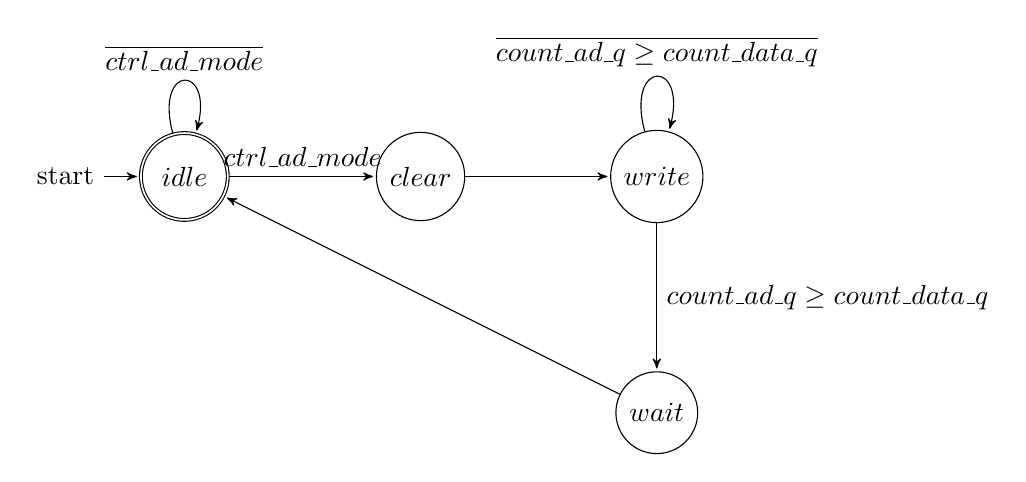
\begin{tikzpicture}[>=stealth',shorten >=1pt,auto,node distance=3cm]
  \node[initial,state,accepting, inner sep=5pt] (idle)   {$idle$};
  \node[state]                   (clear) [right of=idle]  {$clear$};
  \node[state]                   (write) [right of=clear] {$write$};
  \node[state]                   (wait)  [below of=write] {$wait$};

  \path[->]
  (idle)
  edge [loop above]
  node 
  {$\overline{ctrl\_ad\_mode}$} (idle)
  edge
  node 
  {$ctrl\_ad\_mode$} (clear)

  (clear)
  edge 
  node
  {} (write)

  (write)
  edge [loop above]
  node
  {$\overline{count\_ad\_q \geq count\_data\_q}$} (write)
  edge
  node 
  {$count\_ad\_q \geq count\_data\_q$} (wait)

  (wait)
  edge 
  node
  {} (idle)
;
\end{tikzpicture}

\begin{tikzpicture}[>=stealth',shorten >=1pt,auto,node distance=3cm]
  \node[initial,state,accepting, inner sep=5pt] (idle)         {$idle$};
  \node[state]                   (clear) [right of=idle]       {$clear$};
  \node[state]                   (outputlag) [right of=clear]  {$out\_lag$};
  \node[state]                   (write)  [below of=outputlag] {$write$};

  \path[->]
  (idle)
  edge [loop above]
  node 
  {$\overline{write\_enable}$} (idle)
  edge
  node 
  {$write\_enable$} (clear)

  (clear)
  edge 
  node
  {} (outputlag)

  (outputlag)
  edge 
  node
  {} (write)

  (write)
  edge [loop right]
  node
  {$\overline{count\_ram0\_q \geq count\_data\_q}$} (write)
  edge [pos=0.3]
  node 
  {$count\_ram0\_q \geq count\_data\_q$} (idle)

  (wait)
  edge 
  node
  {} (idle)
;
\end{tikzpicture}
\end{document}
